% Chapter 7: Facilitator Service
\chapter{Facilitator Service}
\label{ch:facilitator}

The Facilitator is a critical infrastructure component that handles blockchain interactions on behalf of Resource Servers. It provides verification, settlement, and discovery services while abstracting the complexity of multi-chain operations.

\section{Architecture Overview}
\label{sec:facilitator-architecture}

\begin{figure}[ht]
\centering
\begin{tikzpicture}[
    component/.style={
        rectangle,
        rounded corners=3pt,
        minimum width=2.8cm,
        minimum height=1cm,
        draw=violet,
        line width=1pt,
        fill=violet!10,
        font=\footnotesize\bfseries,
        align=center
    },
    service/.style={
        rectangle,
        rounded corners=2pt,
        minimum width=2cm,
        minimum height=0.6cm,
        draw=blue,
        fill=blue!10,
        font=\tiny,
        align=center
    },
    store/.style={
        cylinder,
        shape border rotate=90,
        aspect=0.3,
        minimum width=1.5cm,
        minimum height=1cm,
        draw=orange,
        fill=orange!10,
        font=\tiny,
        align=center
    }
]

% Main component
\node[component, minimum width=10cm, minimum height=4cm] (facilitator) at (0,0) {};
\node[font=\footnotesize\bfseries, violet] at (0,1.6) {Facilitator Service};

% Internal services
\node[service] (api) at (-3,0.5) {API\\Gateway};
\node[service] (verify) at (0,0.5) {Verification\\Service};
\node[service] (settle) at (3,0.5) {Settlement\\Service};

\node[service] (evm) at (-2,-0.8) {EVM\\Handler};
\node[service] (sol) at (0,-0.8) {Solana\\Handler};
\node[service] (ton) at (2,-0.8) {TON\\Handler};

% External stores
\node[store] (redis) at (-5,0) {Redis};
\node[store] (rpc) at (5,0) {RPC\\Nodes};

% Connections
\draw[->, thick] (api) -- (verify);
\draw[->, thick] (verify) -- (settle);
\draw[->, thick] (verify) -- (evm);
\draw[->, thick] (verify) -- (sol);
\draw[->, thick] (verify) -- (ton);
\draw[->, thick] (settle) -- (evm);
\draw[->, thick] (settle) -- (sol);
\draw[->, thick] (settle) -- (ton);

\draw[<->, thick, gray] (redis) -- (api);
\draw[<->, thick, gray] (rpc) -- (settle);

\end{tikzpicture}
\caption{Facilitator service architecture}
\label{fig:facilitator-architecture}
\end{figure}

\subsection{Core Responsibilities}

\begin{table}[ht]
\centering
\caption{Facilitator Responsibilities}
\label{tab:facilitator-responsibilities}
\begin{tabular}{l p{7cm}}
\toprule
\textbf{Function} & \textbf{Description} \\
\midrule
Verification & Validate signatures, balances, and nonces \\
Settlement & Execute on-chain token transfers \\
Gas Sponsorship & Pay transaction fees on behalf of users \\
Multi-chain & Abstract blockchain-specific details \\
Rate Limiting & Protect against abuse \\
Discovery & Enable resource discovery (Bazaar) \\
\bottomrule
\end{tabular}
\end{table}

\section{API Reference}
\label{sec:facilitator-api}

The Facilitator exposes a RESTful API at \url{https://facilitator.t402.io}.

\subsection{POST /verify}
\label{subsec:verify-endpoint}

Validates a payment authorization without executing on-chain settlement.

\begin{table}[ht]
\centering
\caption{/verify Endpoint}
\label{tab:verify-endpoint}
\begin{tabular}{l l}
\toprule
\textbf{Property} & \textbf{Value} \\
\midrule
Method & POST \\
Content-Type & application/json \\
Rate Limit & 100 requests/minute \\
Timeout & 30 seconds \\
\bottomrule
\end{tabular}
\end{table}

\subsubsection{Request Schema}

\begin{lstlisting}[language=json,caption={/verify request body}]
{
  "paymentPayload": {
    "t402Version": 2,
    "accepted": {
      "scheme": "exact",
      "network": "eip155:8453",
      "asset": "0x833589fCD6eDb6...USDC",
      "amount": "100000",
      "payTo": "0xMerchant..."
    },
    "payload": {
      "from": "0xPayer...",
      "validAfter": 1704067200,
      "validBefore": 1704070800,
      "nonce": "0x7f8a9b0c1d2e3f4a...",
      "signature": "0x2d6a7588ce58f84b..."
    }
  },
  "paymentRequirements": {
    "t402Version": 2,
    "resource": { "url": "https://api.example.com/data" },
    "accepts": [{ ... }]
  }
}
\end{lstlisting}

\subsubsection{Success Response}

\begin{lstlisting}[language=json,caption={/verify success response}]
{
  "isValid": true,
  "payer": "0x857b06519E91e3A54538791bDbb0E22373e36b66",
  "network": "eip155:8453",
  "balance": "1500000",
  "validUntil": 1704070800
}
\end{lstlisting}

\subsubsection{Error Response}

\begin{lstlisting}[language=json,caption={/verify error response}]
{
  "isValid": false,
  "error": {
    "code": "insufficient_funds",
    "message": "Payer has insufficient balance",
    "details": {
      "required": "100000",
      "available": "50000",
      "asset": "USDC"
    }
  }
}
\end{lstlisting}

\subsection{POST /settle}
\label{subsec:settle-endpoint}

Executes the verified payment on the blockchain.

\begin{warningbox}[Idempotency]
Settlement requests are idempotent. If the same nonce is submitted multiple times, only the first will be processed. Subsequent requests return the original transaction hash.
\end{warningbox}

\subsubsection{Request Schema}

\begin{lstlisting}[language=json,caption={/settle request body}]
{
  "paymentPayload": {
    "t402Version": 2,
    "accepted": { ... },
    "payload": { ... }
  },
  "paymentRequirements": { ... }
}
\end{lstlisting}

\subsubsection{Success Response}

\begin{lstlisting}[language=json,caption={/settle success response}]
{
  "success": true,
  "network": "eip155:8453",
  "transaction": "0x7a8b9c0d1e2f3a4b5c6d7e8f9a0b1c2d...",
  "payer": "0x857b06519E91e3A54538791bDbb0E22373e36b66",
  "amount": "100000",
  "asset": "0x833589fCD6eDb6...USDC",
  "blockNumber": 12345678,
  "gasUsed": "65000",
  "effectiveGasPrice": "1000000000"
}
\end{lstlisting}

\subsubsection{Error Response}

\begin{lstlisting}[language=json,caption={/settle error response}]
{
  "success": false,
  "error": {
    "code": "settlement_failed",
    "message": "Transaction reverted",
    "details": {
      "reason": "ERC20: transfer amount exceeds balance",
      "transaction": "0x7a8b9c..."
    }
  }
}
\end{lstlisting}

\subsection{GET /supported}
\label{subsec:supported-endpoint}

Returns supported networks, schemes, and signer addresses.

\begin{lstlisting}[language=json,caption={/supported response}]
{
  "kinds": [
    {
      "t402Version": 2,
      "scheme": "exact",
      "network": "eip155:8453"
    },
    {
      "t402Version": 2,
      "scheme": "exact",
      "network": "eip155:42161"
    },
    {
      "t402Version": 2,
      "scheme": "exact",
      "network": "solana:5eykt4UsFv8P8NJdTREpY1vzqKqZKvdp"
    }
  ],
  "extensions": [
    "subscription",
    "refund"
  ],
  "signers": {
    "eip155:*": ["0xC88f67e776f16DcFBf42e6bDda1B82604448899B"],
    "solana:*": ["8GGtWHRQ1wz5gDKE2KXZLktqzcfV1CBqSbeUZjA7hoWL"],
    "tron:*": ["TT1MqNNj2k5qdGA6nrrCodW6oyHbbAreQ5"]
  },
  "version": "2.0.0"
}
\end{lstlisting}

\subsection{GET /health}
\label{subsec:health-endpoint}

Health check endpoint for monitoring.

\begin{lstlisting}[language=json,caption={/health response}]
{
  "status": "healthy",
  "version": "2.0.0",
  "uptime": 864000,
  "chains": {
    "eip155:8453": {
      "status": "healthy",
      "latency": 45,
      "blockHeight": 12345678
    },
    "eip155:42161": {
      "status": "healthy",
      "latency": 32,
      "blockHeight": 98765432
    },
    "solana:5eykt4UsFv8P8NJdTREpY1vzqKqZKvdp": {
      "status": "degraded",
      "latency": 250,
      "slot": 234567890
    }
  },
  "redis": {
    "status": "healthy",
    "connections": 10
  }
}
\end{lstlisting}

\subsection{GET /metrics}
\label{subsec:metrics-endpoint}

Prometheus-compatible metrics endpoint.

\begin{lstlisting}[caption={/metrics response (Prometheus format)}]
# HELP t402_settlements_total Total settlements
# TYPE t402_settlements_total counter
t402_settlements_total{network="eip155:8453"} 12345
t402_settlements_total{network="eip155:42161"} 6789

# HELP t402_settlement_amount_total Total settled amount
# TYPE t402_settlement_amount_total counter
t402_settlement_amount_total{asset="USDC"} 1234567890000

# HELP t402_verification_duration_seconds Verification time
# TYPE t402_verification_duration_seconds histogram
t402_verification_duration_seconds_bucket{le="0.1"} 9500
t402_verification_duration_seconds_bucket{le="0.5"} 9900
t402_verification_duration_seconds_bucket{le="1.0"} 9990
\end{lstlisting}

\section{Discovery API}
\label{sec:discovery-api}

The Discovery API enables the ``Bazaar'' concept---a decentralized marketplace for T402-enabled resources.

\subsection{GET /discovery/resources}
\label{subsec:discovery-resources}

Lists publicly discoverable T402-enabled resources.

\begin{lstlisting}[language=json,caption={/discovery/resources response}]
{
  "resources": [
    {
      "url": "https://api.example.com/premium",
      "description": "Premium market data API",
      "category": "finance",
      "pricing": {
        "scheme": "exact",
        "amount": "10000",
        "asset": "USDC",
        "networks": ["eip155:8453", "eip155:42161"]
      },
      "provider": {
        "name": "Example Corp",
        "verified": true,
        "rating": 4.8
      },
      "stats": {
        "totalCalls": 1234567,
        "avgLatency": 45
      }
    }
  ],
  "pagination": {
    "page": 1,
    "pageSize": 20,
    "total": 150
  }
}
\end{lstlisting}

\subsection{POST /discovery/register}
\label{subsec:discovery-register}

Register a resource for discovery.

\begin{lstlisting}[language=json,caption={/discovery/register request}]
{
  "url": "https://api.myservice.com/data",
  "description": "Real-time weather data",
  "category": "weather",
  "pricing": {
    "scheme": "exact",
    "amount": "1000",
    "asset": "USDC"
  },
  "signature": "0x..."  // Signed by payTo address
}
\end{lstlisting}

\section{Error Codes}
\label{sec:facilitator-errors}

\begin{longtable}{l l p{5cm}}
\caption{Facilitator Error Codes} \label{tab:facilitator-errors} \\
\toprule
\textbf{Code} & \textbf{HTTP} & \textbf{Description} \\
\midrule
\endfirsthead
\multicolumn{3}{c}{\tablename\ \thetable\ -- continued} \\
\toprule
\textbf{Code} & \textbf{HTTP} & \textbf{Description} \\
\midrule
\endhead
\midrule
\endfoot
\bottomrule
\endlastfoot
\code{invalid\_payload} & 400 & Malformed request body \\
\code{invalid\_signature} & 400 & Signature verification failed \\
\code{invalid\_network} & 400 & Network not supported \\
\code{invalid\_scheme} & 400 & Scheme not supported \\
\code{insufficient\_funds} & 402 & Payer lacks balance \\
\code{nonce\_already\_used} & 409 & Nonce used in prior tx \\
\code{expired\_authorization} & 410 & Authorization expired \\
\code{simulation\_failed} & 422 & Tx simulation failed \\
\code{settlement\_failed} & 500 & On-chain tx failed \\
\code{rate\_limited} & 429 & Too many requests \\
\code{service\_unavailable} & 503 & Temporary outage \\
\end{longtable}

\section{Rate Limiting}
\label{sec:rate-limiting}

The Facilitator implements rate limiting to prevent abuse.

\begin{table}[ht]
\centering
\caption{Rate Limits}
\label{tab:rate-limits}
\begin{tabular}{l l l}
\toprule
\textbf{Endpoint} & \textbf{Limit} & \textbf{Window} \\
\midrule
/verify & 100 requests & 1 minute \\
/settle & 50 requests & 1 minute \\
/supported & 1000 requests & 1 minute \\
/health & Unlimited & -- \\
/discovery/* & 60 requests & 1 minute \\
\bottomrule
\end{tabular}
\end{table}

Rate limit headers are included in responses:

\begin{lstlisting}[caption={Rate limit headers}]
X-RateLimit-Limit: 100
X-RateLimit-Remaining: 95
X-RateLimit-Reset: 1704067260
Retry-After: 45
\end{lstlisting}

\section{Self-Hosting}
\label{sec:self-hosting}

Organizations can deploy their own Facilitator instance for enhanced control and privacy.

\subsection{Requirements}

\begin{table}[ht]
\centering
\caption{Self-Hosting Requirements}
\label{tab:self-hosting-requirements}
\begin{tabular}{l l p{5cm}}
\toprule
\textbf{Component} & \textbf{Minimum} & \textbf{Notes} \\
\midrule
CPU & 2 cores & 4+ for production \\
Memory & 2 GB & 4+ GB recommended \\
Storage & 10 GB & SSD recommended \\
Network & 100 Mbps & Low latency to RPCs \\
\bottomrule
\end{tabular}
\end{table}

\subsection{Hot Wallet Setup}

\begin{warningbox}[Security Critical]
The Facilitator requires a hot wallet with gas funds. Implement proper key management:
\begin{itemize}
    \item Use hardware security modules (HSM) in production
    \item Limit wallet balance to operational needs
    \item Monitor for unauthorized transactions
    \item Implement automated alerts
\end{itemize}
\end{warningbox}

\subsection{Environment Configuration}

\begin{lstlisting}[language=bash,caption={Facilitator environment variables}]
# Server Configuration
PORT=8080
LOG_LEVEL=info
ENVIRONMENT=production

# Network RPC URLs (required)
EVM_RPC_BASE=https://mainnet.base.org
EVM_RPC_ARBITRUM=https://arb1.arbitrum.io/rpc
EVM_RPC_ETHEREUM=https://eth.llamarpc.com
SOLANA_RPC_URL=https://api.mainnet-beta.solana.com
TON_RPC_URL=https://toncenter.com/api/v2
TRON_RPC_URL=https://api.trongrid.io

# Hot Wallet (use HSM in production)
EVM_PRIVATE_KEY=0x...
SOLANA_PRIVATE_KEY=base58...
TRON_PRIVATE_KEY=hex...

# Redis (required for rate limiting)
REDIS_URL=redis://localhost:6379
REDIS_PASSWORD=

# Rate Limiting
RATE_LIMIT_VERIFY=100
RATE_LIMIT_SETTLE=50
RATE_LIMIT_WINDOW=60

# Monitoring
METRICS_ENABLED=true
METRICS_PORT=9090
TRACING_ENABLED=true
JAEGER_ENDPOINT=http://jaeger:14268/api/traces
\end{lstlisting}

\subsection{Docker Deployment}

\begin{lstlisting}[language=yaml,caption={docker-compose.yml}]
version: "3.8"

services:
  facilitator:
    image: ghcr.io/t402-io/facilitator:latest
    ports:
      - "8080:8080"
      - "9090:9090"
    environment:
      - PORT=8080
      - REDIS_URL=redis://redis:6379
      - EVM_RPC_BASE=${EVM_RPC_BASE}
      - EVM_PRIVATE_KEY=${EVM_PRIVATE_KEY}
    depends_on:
      - redis
    healthcheck:
      test: ["CMD", "curl", "-f", "http://localhost:8080/health"]
      interval: 30s
      timeout: 10s
      retries: 3

  redis:
    image: redis:7-alpine
    volumes:
      - redis-data:/data
    command: redis-server --appendonly yes

  prometheus:
    image: prom/prometheus:latest
    volumes:
      - ./prometheus.yml:/etc/prometheus/prometheus.yml
    ports:
      - "9091:9090"

volumes:
  redis-data:
\end{lstlisting}

\subsection{Kubernetes Deployment}

\begin{lstlisting}[language=yaml,caption={Kubernetes Deployment manifest}]
apiVersion: apps/v1
kind: Deployment
metadata:
  name: facilitator
  labels:
    app: facilitator
spec:
  replicas: 3
  selector:
    matchLabels:
      app: facilitator
  template:
    metadata:
      labels:
        app: facilitator
    spec:
      containers:
      - name: facilitator
        image: ghcr.io/t402-io/facilitator:latest
        ports:
        - containerPort: 8080
        - containerPort: 9090
        envFrom:
        - secretRef:
            name: facilitator-secrets
        - configMapRef:
            name: facilitator-config
        resources:
          requests:
            memory: "512Mi"
            cpu: "500m"
          limits:
            memory: "2Gi"
            cpu: "2000m"
        livenessProbe:
          httpGet:
            path: /health
            port: 8080
          initialDelaySeconds: 10
          periodSeconds: 30
        readinessProbe:
          httpGet:
            path: /health
            port: 8080
          initialDelaySeconds: 5
          periodSeconds: 10
\end{lstlisting}

\section{Monitoring and Observability}
\label{sec:monitoring}

\subsection{Key Metrics}

\begin{table}[ht]
\centering
\caption{Critical Monitoring Metrics}
\label{tab:monitoring-metrics}
\footnotesize
\begin{tabular}{l l p{4.5cm}}
\toprule
\textbf{Metric} & \textbf{Type} & \textbf{Alert Threshold} \\
\midrule
Settlement success rate & Gauge & $<$ 99\% \\
Verification latency p99 & Histogram & $>$ 500ms \\
Settlement latency p99 & Histogram & $>$ 30s \\
Hot wallet balance & Gauge & $<$ \$100 equivalent \\
RPC error rate & Counter & $>$ 1\% \\
Rate limit hits & Counter & $>$ 100/min \\
\bottomrule
\end{tabular}
\end{table}

\subsection{Grafana Dashboard}

A pre-built Grafana dashboard is available at:

\begin{center}
\url{https://grafana.facilitator.t402.io}
\end{center}

\begin{figure}[ht]
\centering
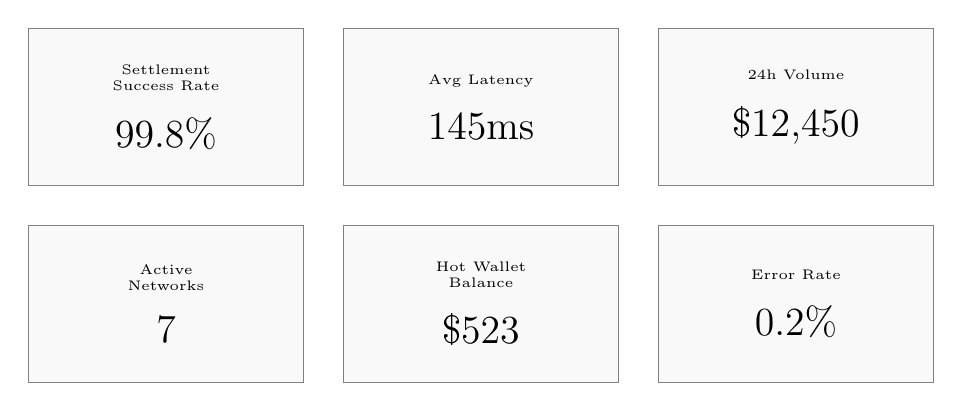
\begin{tikzpicture}[
    panel/.style={
        rectangle,
        minimum width=3.5cm,
        minimum height=2cm,
        draw=gray,
        fill=gray!5,
        font=\tiny,
        align=center
    }
]

\node[panel] at (0,0) {Settlement\\Success Rate\\[0.3cm]\Large 99.8\%};
\node[panel] at (4,0) {Avg Latency\\[0.3cm]\Large 145ms};
\node[panel] at (8,0) {24h Volume\\[0.3cm]\Large \$12,450};
\node[panel] at (0,-2.5) {Active\\Networks\\[0.3cm]\Large 7};
\node[panel] at (4,-2.5) {Hot Wallet\\Balance\\[0.3cm]\Large \$523};
\node[panel] at (8,-2.5) {Error Rate\\[0.3cm]\Large 0.2\%};

\end{tikzpicture}
\caption{Grafana dashboard overview}
\label{fig:grafana-dashboard}
\end{figure}

\subsection{Alerting Rules}

\begin{lstlisting}[language=yaml,caption={Prometheus alerting rules}]
groups:
- name: facilitator
  rules:
  - alert: HighSettlementFailureRate
    expr: |
      rate(t402_settlements_total{status="failed"}[5m])
      / rate(t402_settlements_total[5m]) > 0.01
    for: 5m
    labels:
      severity: critical
    annotations:
      summary: "Settlement failure rate > 1%"

  - alert: LowWalletBalance
    expr: t402_wallet_balance_usd < 100
    for: 1m
    labels:
      severity: warning
    annotations:
      summary: "Hot wallet balance low"

  - alert: HighVerificationLatency
    expr: |
      histogram_quantile(0.99,
        rate(t402_verification_seconds_bucket[5m])
      ) > 0.5
    for: 10m
    labels:
      severity: warning
    annotations:
      summary: "p99 verification latency > 500ms"
\end{lstlisting}

\section{Security Considerations}
\label{sec:facilitator-security}

\subsection{Authentication}

For self-hosted deployments, implement API authentication:

\begin{lstlisting}[language=bash,caption={API key authentication}]
# Request with API key
curl -X POST https://facilitator.example.com/verify \
  -H "Authorization: Bearer sk_live_abc123..." \
  -H "Content-Type: application/json" \
  -d '{"paymentPayload": {...}}'
\end{lstlisting}

\subsection{Network Security}

\begin{itemize}
    \item Deploy behind a reverse proxy (nginx, Cloudflare)
    \item Enable TLS 1.3 only
    \item Implement IP allowlisting for /settle endpoint
    \item Use private networking for Redis connections
    \item Rotate API keys regularly
\end{itemize}

\subsection{Audit Logging}

All settlement operations are logged with:

\begin{lstlisting}[language=json,caption={Audit log entry}]
{
  "timestamp": "2026-01-15T10:30:00Z",
  "event": "settlement",
  "network": "eip155:8453",
  "transaction": "0x7a8b9c...",
  "payer": "0x857b06...",
  "payTo": "0xMerchant...",
  "amount": "100000",
  "asset": "USDC",
  "gasUsed": "65000",
  "clientIP": "192.168.1.100",
  "userAgent": "T402-Server/2.0"
}
\end{lstlisting}

\section{Operational Runbook}
\label{sec:runbook}

\subsection{Common Issues}

\begin{table}[ht]
\centering
\caption{Troubleshooting Guide}
\label{tab:troubleshooting}
\footnotesize
\begin{tabular}{p{3cm} p{4cm} p{4cm}}
\toprule
\textbf{Symptom} & \textbf{Cause} & \textbf{Resolution} \\
\midrule
High verification latency & RPC congestion & Switch to backup RPC \\
Settlement failures & Low gas balance & Refill hot wallet \\
Rate limit errors & Traffic spike & Scale horizontally \\
Nonce errors & Concurrent txs & Implement nonce manager \\
\bottomrule
\end{tabular}
\end{table}

\subsection{Emergency Procedures}

\begin{enumerate}
    \item \textbf{Service Degradation}: Enable circuit breaker, switch to backup RPCs
    \item \textbf{Wallet Compromise}: Immediately rotate keys, pause settlements
    \item \textbf{Chain Outage}: Mark chain as unhealthy, inform users
    \item \textbf{Data Breach}: Rotate all API keys, audit access logs
\end{enumerate}

